\chapter{锁}\label{ch06}

包括xv6在内的大多数内核都交错执行多个活动。
交错执行的一个原因是多处理器硬件:有多个独立执行计算等等CPU的计算机,例如xv6的RISC-V。
这些CPU会共享物理RAM,xv6利用这种共享来维护所有CPU读写的数据结构。
这种共享导致了可能会有一个CPU正在读取一个数据结构,而同时还有另一个CPU也正在更新它,或者多个CPU同时更新同一个数据。
如果没有精心的设计,这种并行访问可能会返回错误的结果或者破坏数据结构。
即使在一个单处理器上,内核也可能在多个线程间切换CPU,导致它们的执行是交错的。
最后,设备中断处理程序可能和被中断的代码修改同一个数据,如果中断恰好在错误的时间发生就可能破坏数据。
单词\emph{并发(concurrency)}指多个指令流交错执行的情况,可能是因为多处理器并行、线程切换或者中断。

内核中充满了并发访问的数据。
例如,两个CPU可能会同时调用\texttt{kalloc},因此它们会并发地从空闲列表的头部移除节点。
内核设计者更喜欢允许很多并发,因为这样可以通过并行提高性能和响应能力。
然而,内核设计者必须确保这种并发的正确性。
有很多种方法可以写出正确的代码,其中一些比另外一些更加容易理解。
致力于在并发中保持正确性的策略,以及支撑这些策略的概念,被称之为\emph{并发控制(concurrency control)}技术。

xv6根据具体情况使用了很多并发控制技术,还有可能使用更多。
这一章聚焦于一个被广泛使用的技术:\emph{锁(lock)}。
锁提供了相互排斥性,确保了某一个时间点只有一个CPU可以持有这个锁。
如果程序员把一个锁和一些共享数据联系起来,并且代码总是在使用数据的时候持有相关的锁,那么这个数据在任何时间点都只被一个CPU使用。
在这种情况下,我们说锁保护了这个数据。
尽管锁是非常容易理解的并发控制机制,但锁的弊端是它们可能会限制性能,因为它们把并发的操作串行化了。

本章的剩余部分将解释为什么xv6需要锁、xv6如何实现锁、以及如何使用它们。

\section{竞争}
我们用一个例子来说明为什么我们需要锁,考虑有两个进程正在两个不同的CPU上调用\texttt{wait}等待它们刚结束的子进程。
\texttt{wait}会释放子进程的内存,因此在每个CPU上,内核都会调用\texttt{kfree}去释放子进程的内存页。
内核分配器维护了一个链表:\texttt{kalloc()}\href{https://github.com/mit-pdos/xv6-riscv/blob/riscv//kernel/kalloc.c#L69}{(kernel/kalloc.c:69)}从空闲页链表中弹出一个内存页,\texttt{kfree()}\href{https://github.com/mit-pdos/xv6-riscv/blob/riscv//kernel/kalloc.c#L47}{(kernel/kalloc.c:47)}把一个页放进空闲列表。
为了最好的性能,我们可能会希望两个附近承德\texttt{kfree}能并行执行,无需等待彼此,但对xv6的\texttt{kfree}实现来说这样可能会导致错误的结果。

\begin{figure}[htbp]
    \centering
    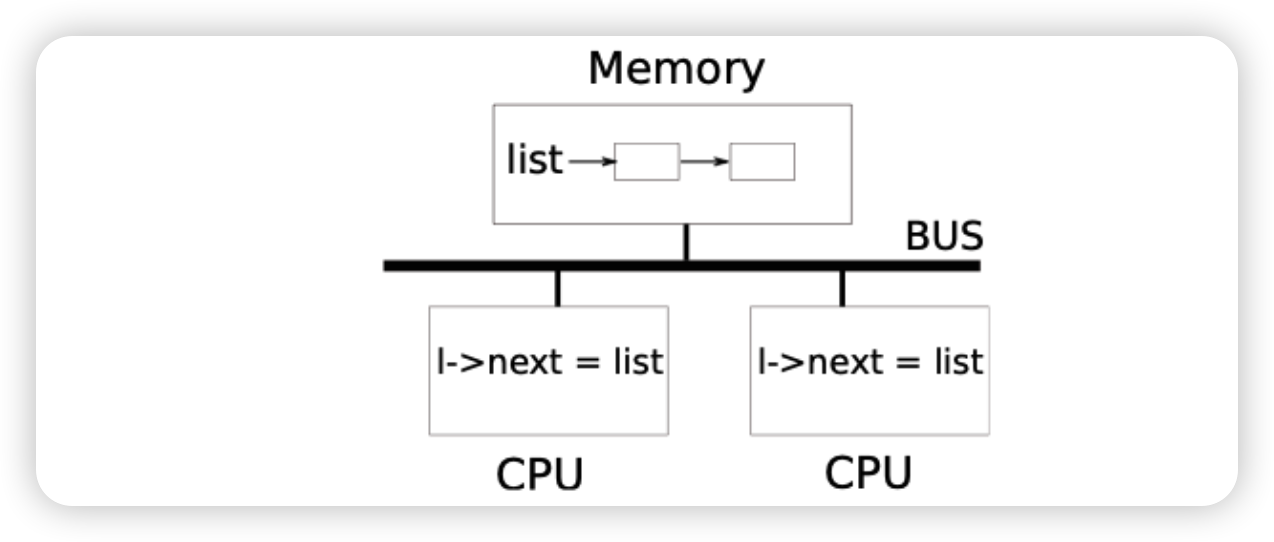
\includegraphics[width=0.8\textwidth]{../imgs/f6-1.png}
    \caption{简化的SMP架构}
    \label{f6-1}
\end{figure}

\autoref{f6-1}更加详细地演示了这个过程:空闲页的链表所在的内存被两个CPU共享,这两个CPU使用load和store指令操作链表。
(实际上,处理器是有缓存的,但概念上多处理器系统表现得好像只有单个共享的内存。)
如果没有并发的请求,你可以像下面这样实现链表的\texttt{push}操作:
\begin{lstlisting}[numbers=left]
    struct element {
        int data;
        struct element *next;
    };

    struct element *list = 0;

    void
    push(int data)
    {
        struct element *l;
        l = malloc(sizeof *l);
        l->data = data;
        l->next = list;
        list = l;
    }
\end{lstlisting}

这段代码如果在隔离的环境下执行,那么它是正确的。
然而,如果有多个副本同时执行,那么它是错误的。
如果两个CPU同时执行\texttt{push},可能会像\author{f6-1}所示一样同时执行第15行,这会导致如\autoref{f6-2}所示的错误结果。
将会有两个链表元素的\texttt{next}都被设成\texttt{list}一开始的值。
当到达第16行时两个CPU都会给\texttt{list}赋值,第二次赋值将会覆盖第一次赋值,参与第一次赋值的元素将会丢失。

\begin{figure}[htbp]
    \centering
    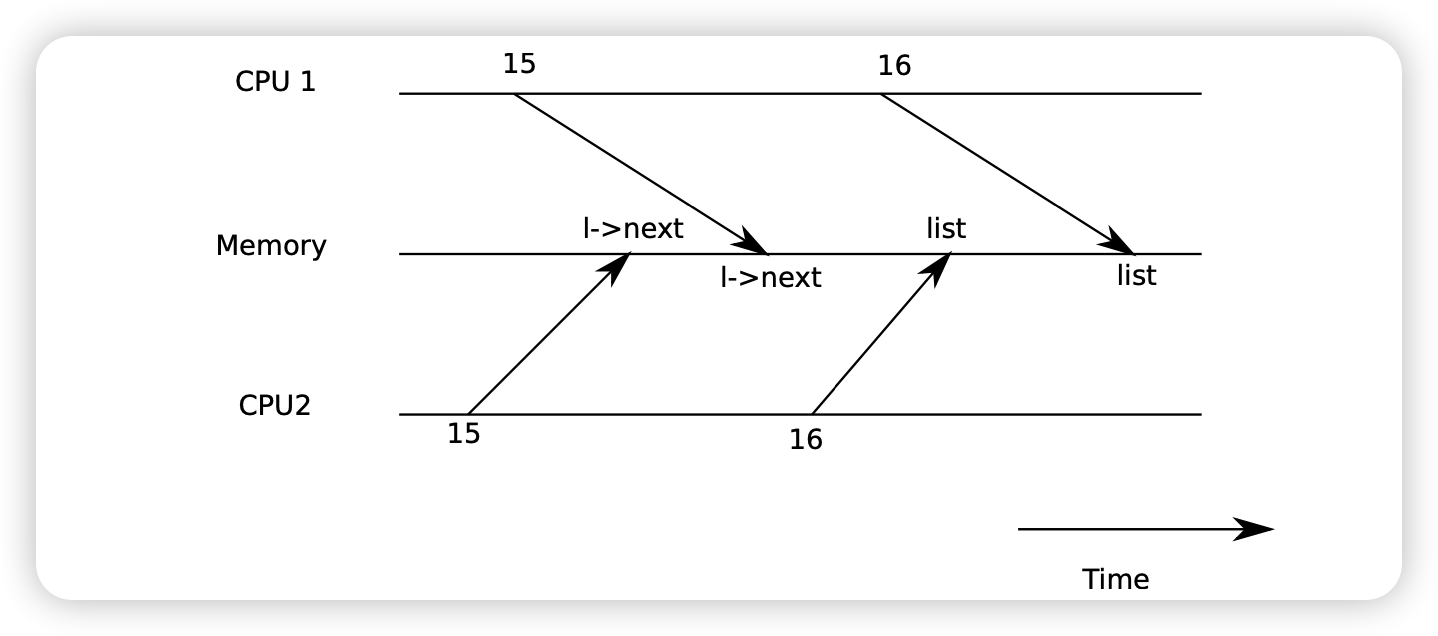
\includegraphics[width=0.8\textwidth]{../imgs/f6-2.png}
    \caption{竞争示例}
    \label{f6-2}
\end{figure}

第16行的更新丢失是\emph{竞争(race)}的一个例子。
竞争是指一个内存位置被并发访问,其中至少一个访问是写入操作。
竞争通常是bug的标志,可能是更新丢失(如果访问都是写入)或者读取到还未完全更新的数据结构。
竞争的结果取决于编译器生成的机器代码、两个CPU执行的时间、以及内存系统如何为它们的内存操作排序,这些都可能导致竞争产生的错误难以复现和调试。
例如,在调试\texttt{push}的时候添加和一条输出语句就可能改变执行的时间,进而导致竞争消失。

避免竞争的通常方法是锁。
锁保证了\emph{相互排斥(mutual exclusion)},因此同一时刻只有一个CPU能执行\texttt{push}中的敏感行,这让上面的场景变得不可能再发生。
上面的代码的正确加锁版本只需要添加几行(第7、16、19行):
\begin{lstlisting}[numbers=left,firstnumber=6]
    struct element *list = 0;
    struct lock listlock;

    void 
    push(int data)
    {
        struct element *l;
        l = malloc(sizeof *l);
        l->data = data;
        
        acquire(&listlock);
        l->next = list;
        list = l;
        release(&listlock);
    }
\end{lstlisting}

\texttt{acquire}和\texttt{release}之间的指令序列通常被称为\emph{临界区(critical section)}。
通常说锁保护了\texttt{list}。

当我们说锁保护数据时,我们实际上是在说锁保护了适用于这个数据的一些不变量的集合。
不变量是数据结构在多个操作间维护的属性。
通常情况下,一个操作的行为正确依赖于操作开始时不变量为真。
操作可能会临时违反不变量但最终会在结束之前恢复。
例如,在这个列表的例子中,不变量是\texttt{list}指向链表中的第一个元素并且每个元素的\texttt{next}字段指向下一个元素。
\texttt{push}的实现短暂违反了不变量:在第17行,\texttt{l}指向了下一个链表元素,但\texttt{list}还没有指向\texttt{l}(在第18行恢复了不变量)。
我们之前讨论的竞争会发生是因为第二个CPU执行代码时依赖于链表的不变量,但它们被(临时地)违反了。
恰当地使用锁可以确保同一时刻在临界区内只有一个CPU可以操作数据结构,因此在数据结构的不变量不成立时不会有其他CPU操作这个数据结构。

你可以把锁看成\emph{串行化(serializing)}了临界区,所以它们只能同时运行一个,因此保证了不变量(假设临界区在隔离环境中是正确的)。
你也可以想象成被同一个锁保护的临界区是原子的,因此每个CPU只能看到其他CPU执行完临界区之后的变化,而不能看到部分执行时的变化。

尽管锁在确保正确性时非常有用,但它会潜在地限制性能。
例如,如果两个进程并发调用\texttt{kfree},锁将会串行化两个临界区,因此将不能受益于在不同CPU上执行它们。
如果两个进程同时想获取同一个锁,我们说这两个进程\emph{冲突(conflict)}了,或者说锁遇到了\emph{争用(contention)}。
内核设计中一个主要的挑战就是如何在追求并行性的同时避免锁的争用。
xv6在这方面只作了很少的工作,但成熟的内核通过特殊地组织内核数据结构和算法来避免争用。
在链表的例子中,内核可以为每个CPU维护一个单独的空闲链表,并只有在当前CPU的链表为空,需要从其他CPU那里偷取内存时才会访问另一个CPU的空闲链表。
其他的用例可能会需要更加复杂的设计。

放置锁的位置也会严重影响到性能。
例如,如果把\texttt{acquire}移动到\texttt{push}之前,也就是13行之前,那么代码也是正确的。
但这可能会降低性能因为这样的话对\texttt{malloc}的调用也会串行化。
“使用锁”这一节中将会提供一些在哪里插入\texttt{acquire}和\texttt{release}的指导意见。

\section{代码:锁}
xv6有两种锁:自旋锁和睡眠锁。
我们将以自旋锁开始。
xv6用\texttt{struct spinlock}\href{https://github.com/mit-pdos/xv6-riscv/blob/riscv//kernel/spinlock.h#L2}{(kernel/spinlock.h:2)}表示自旋锁。
这个结构体中比较重要的字段是\texttt{locked},当锁可用时它的值是0,当已经被持有时值为1。
逻辑上讲,xv6应该执行类似这样的代码来获取一个锁
\begin{lstlisting}[numbers=left,firstnumber=21]
    void
    acquire(struct spinlock *lk) // does not work!
    {
        for (;;) {
            if (lk->locked == 0) {
                lk->locked = 1;
                break;
            }
        }
    }
\end{lstlisting}
不幸的是,这种实现在多处理器上并不能保证互斥。
两个CPU可能会同时到达第25行,然后发现\texttt{lk->locked}是0,然后都执行第26行获取锁。
这时,两个不同的CPU都持有了这个锁,这违背了互斥的属性。
我们需要的是把第25行和第26行做为一个\emph{原子(atomic)}(即不可分割)的步骤执行。

因为锁被广泛使用,多核处理器通常提供第25行和第26行的一个原子版本。
在RISC-V上这个指令是\texttt{amoswap r, a}。
\texttt{smoswap}读取内存地址\texttt{a}处的值,把寄存器\texttt{r}的内容写入这个地址,再把读取到的值写入\texttt{r}。
也就是说,它交换了寄存器和内存地址处的值。
它以原子的方式执行这一系列操作,使用特殊的硬件来防止任何其他的CPU在它读写过程中使用这个内存地址。

xv6的\texttt{acquire}\href{https://github.com/mit-pdos/xv6-riscv/blob/riscv//kernel/spinlock.c#L22}{(kernel/spinlock.c:22)}使用了可移植的C库调用\texttt{\_\_sync\_lock\_test\_and\_set},它会转换为\texttt{amoswap}指令,返回值是之前的(被交换的)\texttt{lk->locked}的内容。
\texttt{acquire}函数把这个交互包装在了一个循环中,尝试(自旋)直到它获取锁。
每一次迭代都把1和\texttt{lk->locked}交换然后检查\texttt{lk->locked}之前的值,如果之前的值是0,那么就说明已经获取锁了,然后这一次交互已经把\texttt{lk->locked}设置为1了。
如果之前的值是1,那么说明其他的CPU持有了这个锁,我们原子地把1交换进\texttt{lk->locked}并不会改变它的值。

一旦获取了锁,\texttt{acquire}会记录下CPU获取了这个锁(为了调试)。
\texttt{lk->cpu}字段被锁保护并只能在持有锁的时候修改。

函数\texttt{release}\href{https://github.com/mit-pdos/xv6-riscv/blob/riscv//kernel/spinlock.c#L47}{(kernel/spinlock.c:47)}和\texttt{acquire}相反:它清空\texttt{lk->cpu}字段,然后释放锁。
概念上讲,释放操作只需要把0赋值给\texttt{lk->locked}。
C标准允许编译器用多条store指令实现赋值操作,因此一条C赋值语句可能不是原子的。
作为代替,\texttt{release}使用了C库函数\texttt{\_\_sync\_lock\_release}来进行原子的赋值。
这个函数也会转换为RISC-V的\texttt{amoswap}指令。

\section{代码:使用锁}
xv6在很多地方使用锁来避免竞争。
正如之前说的,\texttt{kalloc}\href{https://github.com/mit-pdos/xv6-riscv/blob/riscv//kernel/kalloc.c#L69}{(kernel/kalloc.c:69)}和\texttt{kfree}\href{https://github.com/mit-pdos/xv6-riscv/blob/riscv//kernel/kalloc.c#L47}{(kernel/kalloc.c:47)}就是一个很好的例子。
尝试练习1和2来搞清楚如果这些函数省略了锁会发生什么。
你可能会发现很难触发错误的行为,记住想要可靠地测试处代码是否没有锁错误和竞争是非常困难的。
xv6中很可能也还有未被发现的竞争。

锁的使用中比较困难的一点是决定要使用多少锁以及每个锁应该保护哪些数据和不变量。
有一些基本的原则。
首先,任何时候如果有一个变量在被一个CPU写入的同时可能会有另一个CPU读取或写入它,那么应该使用一个锁来保证两个CPU的操作不会重叠。
第二,记住锁是用来保护不变量的:如果一个不变量涉及到了多个内存位置,通常它们应该被单个锁保护以确保可以维持不变量。

上面的规则描述了什么时候锁是必要的,但并没有说什么时候锁不是必要的,不使用过多锁对保证性能来说是很重要的,因为锁会降低并行性。
如果并行性不重要,那么你可以只使用单个线程,这样就不需要担心锁了。
一个简单的内核可以在多处理器上只使用单个锁做到这一点:进入内核的时候必须获取这个锁,离开内核的时候必须释放它(尽管阻塞像管道读取或者\texttt{wait}这样的系统调用可能会有问题)。
很多单处理器操作系统就是使用这种方式转换成了在多处理器上运行,有时也称为“大内核锁”。
但这种方式牺牲了并行性:任何时刻只有一个CPU可以在内核中执行。
如果内核中要进行大量计算,使用一组更加细粒度的锁将会更加高效,这样内核可以同时在多个CPU上执行。

作为粗粒度锁的一个例子,xv6的\texttt{kalloc.c}分配器使用了被单个锁保护的单个空闲链表。
如果不同CPU上的多个进程同时尝试分配内存,每一个都不得不通过在\texttt{acquire}中自旋以等待轮到它们的时候。
自旋会浪费CPU时间,因为它并不是有效的工作。
如果锁的争用浪费了很大一部分CPU时间,那么可能可以通过把分配器的设计修改为有多个空闲链表、每个都有自己的锁、允许真正并行的分配来提高性能。

作为细粒度锁的一个例子,xv6为每个文件有一个单独的锁,因此操作不同文件的进程通常可以无需等待彼此的锁继续执行。
如果想要允许多个进程同时写入同一个文件的不同区域,那么文件的锁定方案还可以更加细粒度一些。
到最后,锁的粒度的决策需要由性能测试来驱动,也还需要考虑复杂性。

随后的章节会解释xv6的每一部分,它们都会提到xv6使用锁来处理并发的例子。
作为预览,\autoref{t6-1}列出了xv6中的所有锁。

\begin{table}[htbp]
    \centering
    \begin{tabular}{l|l}
        \textbf{锁}     & \textbf{描述} \\
        \hline
        bcache.lock     & 保护块缓冲区cache条目的分配   \\
        cons.lock       & 序列化对控制台硬件的访问,避免交错的输出  \\
        ftable.lock     & 序列化文件表中结构文件的分配  \\
        itable.lock     & 保护内存中inode条目的分配     \\
        vdisk\_lock     & 序列化对磁盘硬件和DMA描述符队列的访问     \\
        kmem.lock       & 序列化内存的分配      \\
        log.lock        & 序列化对事务日志的操作    \\
        管道的pi->lock   & 序列化对每个管道的操作    \\
        pid\_lock       & 序列化\texttt{next\_pid}的递增    \\
        进程的p->lock    & 序列化对进程状态的更改   \\
        wait\_lock      & 帮助wait避免丢失的唤醒\footnote{todo!}    \\
        tickslock       & 序列化对tick计数器的操作  \\
        inode的ip->lock & 序列化对每个inode和它的内容的操作 \\
        缓冲区的b->lock  & 序列化对每个块缓冲区的操作   \\
    \end{tabular}
    \caption{xv6中的锁}
    \label{t6-1}
\end{table}

\section{死锁和加锁顺序}
如果内核里的一段代码执行路径必须同时持有多个锁,那么确保所有代码路径都按照同样的顺序获取这些锁是很重要的。
否则,就会有\emph{死锁(deadlock)}的风险。
假设xv6中有两段代码路径都需要获取锁A和B,但代码路径1先获取A再获取B,而代码路径2先获取B再获取A。
假设线程T1执行代码路径1并且已经获取了锁A,线程T2执行代码路径2并且已经获取了锁B。
接下来T1将会尝试获取锁B,而T2将会尝试获取锁A。
这两个获取锁的操作都会无限阻塞下去,因为另一个线程持有了它需要的锁,并且在获取操作返回之前不会释放这个锁。
为了避免这种死锁,所有的代码路径必须按照同样的顺序获取锁。
需要这种全局的锁获取顺序意味着锁实际上是每个函数规范的一部分:调用者必须以一种按照指定顺序获取锁的方式调用函数。

因为\texttt{sleep}的工作方式(\autoref{ch07}),xv6有很多获取两个每个进程的锁(每个\texttt{struct proc}中的锁)的顺序。
例如,\texttt{consoleintr}\href{https://github.com/mit-pdos/xv6-riscv/blob/riscv//kernel/console.c#L136}{(kernel/console.c:136)}是处理输入字符的中断处理程序。
当有一个换行符到达时,任何等待控制台输入的进程都应该被唤醒。
为了做到这一点,\texttt{consoleintr}在调用\texttt{wakeup}时会持有\texttt{cons.lock},这个函数会获取正在等待的进程的锁以便唤醒它。
全局的避免死锁加锁顺序包括了\texttt{cons.lock}必须在任何进程锁被获取之前先被获取。
文件系统的代码包含了xv6中最长的加锁链。
例如,创建一个文件需要同时持有目录的锁、新文件i节点的锁、磁盘块缓冲区的锁、磁盘驱动的\texttt{vdisk\_lock}、调用进程的\texttt{p->lock}。
为了避免死锁,文件系统的总是按照上面提到的顺序来加锁。

全局的避免死锁顺序可能会出乎意料的难。
有时加锁顺序会和程序的逻辑结构冲突,例如一个代码模块M1会调用模块M2,但加锁顺序要求M2中的锁必须比M1中的锁先被获取。
有时并不能提前知道要获取哪一个锁,可能是因为必须持有一把锁之后才能发现接下来要获取哪个锁。
这种情况在文件系统中就会出现,因为它需要在一个路径名中查找多个连续的组件,在\texttt{wait}和\texttt{exit}的代码中也会出现,因为它要查找子进程的进程表。
最后,死锁的风险通常是锁定方案可以做到多小粒度的一个约束,因为更多的锁通常意味着死锁的风险会更大。
避免死锁通常是内核设计中的一个主要因素。

\section{可重入锁}
通过使用\emph{可重入锁(re-entrant lock)}可以避免一些死锁和加锁顺序的挑战,它也被称为\emph{递归锁(recursive lock)}。
它的关键思路是如果它已经被一个进程持有了,并且这个进程再次尝试获取它,那么内核会允许这一次获取(因为这个进程已经持有这个锁了),而不是调用panic,xv6就是这么做的。

然而事实证明,可重入锁让并发变得更加难以理解:可重入锁打破了锁可以让临界区变为原子的这一特点。
考虑下面的两个函数\texttt{f}和\texttt{g}:
\begin{lstlisting}
    struct spinlock lock;
    int data = 0;   // 被锁保护
    
    f() {
        acquire(&lock);
        if (data == 0) {
            call_once();
            h();
            data = 1;
        }
        release(&lock);
    }

    g() {
        acquire(&lock);
        if (data == 0) {
            call_once();
            data = 1;
        }
        release(&lock);
    }
\end{lstlisting}

这个代码片段中,直觉上好像\texttt{call\_once}只会被调用一次:要么被\texttt{f}调用,要么被\texttt{g}调用,而不会两个都调用。

但如果允许可重入锁,并且\texttt{h}恰好调用了\texttt{g},那么\texttt{call\_once}可能会被调用\emph{两次}。

如果不允许可重入锁,那么\texttt{h}调用\texttt{g}会导致死锁,这同样也不好。
但是,假如调用\texttt{call\_once}两次会产生非常严重的错误,那么死锁可能会更好一点。
内和开发者将会观测到这个死锁(内核会panic)并且修复代码来避免它,然而调用\texttt{call\_once}两次可能无声无息地导致难以追踪的错误。

出于这个原因,xv6使用了更易于理解的非重入锁。
不过,只要程序员时刻谨记加锁的规则,每种方案都可以正常工作。
如果xv6使用可重入锁,那么需要修改\texttt{acquire}让它注意锁是否已经被当前线程持有了。
可能还需要给spinlock结构体添加一个嵌套获取次数的计数器,类似于之后要讨论的\texttt{push\_off}。

\section{锁和中断处理程序}\label{s6-6}
一些xv6的自旋锁被用来保护那些同时被线程和中断处理程序使用的数据。
例如,\texttt{clockintr}时钟中断处理程序可能会递增\texttt{ticks}\href{https://github.com/mit-pdos/xv6-riscv/blob/riscv//kernel/trap.c#L164}{(kernel/trap.c:164)},同时内核线程也可能在\texttt{sys\_sleep}\href{https://github.com/mit-pdos/xv6-riscv/blob/riscv//kernel/sysproc.c#L59}{(kernel/sysproc.c:59)}中读取\texttt{ticks}。
\texttt{tickslock}锁序列化了这两个访问。

自旋锁和中断的相互作用引入了一个潜在的风险。
假设\texttt{sys\_sleep}持有了\texttt{tickslock},并且它的CPU被一个时钟中断中断。
那么\texttt{clockintr}将会尝试获取\texttt{tickslock},然后发现它已经被持有了,就开始等待它被释放。
在这种情况下,\texttt{tickslock}将永远不会被释放:只有\texttt{sys\_sleep}可以释放它,但是\texttt{sys\_sleep}将直到\texttt{clockintr}返回时才能继续执行。
因此CPU会死锁,并且任何需要加锁的代码也会冻结。

为了避免这种情况,如果在中断处理程序使用了自旋锁,那么CPU决不能在允许中断的情况下持有它。
xv6更加保守:当一个CPU获取任何锁时,xv6总是会禁用那个CPU上的中断。
中断仍然可能出现在其他CPU上,因此中断的\texttt{acquire}可能还是会等待一个线程释放一个自旋锁,不过不是在同一个CPU上。

xv6在CPU不持有自旋锁时重新启用中断,它必须做一些簿记来处理嵌套的临界区。
\texttt{acquire}调用\texttt{push\_off}\href{https://github.com/mit-pdos/xv6-riscv/blob/riscv//kernel/spinlock.c#L89}{(kernel/spinlock.c:89)}、\texttt{release}调用\texttt{pop\_off}\href{https://github.com/mit-pdos/xv6-riscv/blob/riscv//kernel/spinlock.c#L100}{(kernel/spinlock.c:100)}来追踪当前CPU上锁的嵌套层级。
当计数为0时,\texttt{pop\_off}会恢复最外层临界区开始时中断的启用状态。
\texttt{intr\_off}和\texttt{intr\_on}函数执行RISC-V执行来分别禁用和启用中断。

重要的一点是\texttt{acquire}必须在设置\texttt{lk->locked}\href{https://github.com/mit-pdos/xv6-riscv/blob/riscv//kernel/spinlock.c#L28}{(kernel/spinlock.c:28)}之前调用\texttt{push\_off}。
如果顺序反了,将会有一个很短的窗口期,此时锁已经被持有了,而中断还是启用的状态,此时如果不行发生时钟中断可能会导致系统死锁。
类似地,\texttt{release}在释放锁\href{https://github.com/mit-pdos/xv6-riscv/blob/riscv//kernel/spinlock.c#L66}{(kernel/spinlock.c:66)}之后调用\texttt{pop\_off}也很重要。

\section{指令和内存顺序}

